%%
%% ConcurrencyLab (c) 2021 Christopher A. Bohn
%%
%% Licensed under the Apache License, Version 2.0 (the "License");
%% you may not use this file except in compliance with the License.
%% You may obtain a copy of the License at
%%     http://www.apache.org/licenses/LICENSE-2.0
%% Unless required by applicable law or agreed to in writing, software
%% distributed under the License is distributed on an "AS IS" BASIS,
%% WITHOUT WARRANTIES OR CONDITIONS OF ANY KIND, either express or implied.
%% See the License for the specific language governing permissions and
%% limitations under the License.
%%

%%
%% (c) 2021 Christopher A. Bohn
%%

\documentclass[12pt]{article}

\usepackage{fullpage}
\usepackage{fancyhdr}
\usepackage[procnames]{listings}
\usepackage{hyperref}
\usepackage{textcomp}
\usepackage{bold-extra}
\usepackage[dvipsnames]{xcolor}
\usepackage{etoolbox}


% Customize the semester (or quarter) and the course number

\newcommand{\courseterm}{Spring 2022}
\newcommand{\coursenumber}{CSCE 231}

% Customize how a typical lab will be managed;
% you can always use \renewcommand for one-offs

\newcommand{\runtimeenvironment}{your account on the \textit{csce.unl.edu} Linux server}
\newcommand{\filesource}{Canvas or {\footnotesize$\sim$}cse231 on \textit{csce.unl.edu}}
\newcommand{\filesubmission}{Canvas}

% These are placeholder commands and will be renewed in each lab

\newcommand{\labnumber}{}
\newcommand{\labname}{Lab \labnumber\ Assignment}
\newcommand{\shortlabname}{}
\newcommand{\duedate}{}

% Individual or team effort

\newcommand{\individualeffort}{This is an individual-effort project. You may discuss concepts and syntax with other students, but you may discuss solutions only with the professor and the TAs. Sharing code with or copying code from another student or the internet is prohibited.}
\newcommand{\teameffort}{This is a team-effort project. You may discuss concepts and syntax with other students, but you may discuss solutions only with your assigned partner(s), the professor, and the TAs. Sharing code with or copying code from a student who is not on your team, or from the internet, is prohibited.}
\newcommand{\freecollaboration}{In addition to the professor and the TAs, you may freely seek help on this assignment from other students.}
\newcommand{\collaborationrules}{}

% Do you care about software engineering?

\providebool{allowspaghetticode}

\setbool{allowspaghetticode}{false}

\newcommand{\softwareengineeringfrontmatter}{
    \ifboolexpe{not bool{allowspaghetticode}}{
        \section*{No Spaghetti Code Allowed}
        In the interest of keeping your code readable, you may \textit{not} use
        any \lstinline{goto} statements, nor may you use any \lstinline{break}
        statements to exit from a loop, nor may you have any functions
        \lstinline{return} from within a loop.
    }{}
}

\newcommand{\spaghetticodepenalties}[1]{
    \ifboolexpe{not bool{allowspaghetticode}}{
        \penaltyitem{1}{for each \lstinline{goto} statement, \lstinline{break}
            statement used to exit from a loop, or \lstinline{return} statement
            that occurs within a loop.}
    }{}
}

% You shouldn't need to customize these,
% but you can if you like

\lstset{language=C, tabsize=4, upquote=true, basicstyle=\ttfamily}
\newcommand{\function}[1]{\textbf{\lstinline{#1}}}
\setlength{\headsep}{0.7cm}
\hypersetup{colorlinks=true}

\newcommand{\startdocument}{
    \pagestyle{fancy}
    \fancyhf{}
    \lhead{\coursenumber}
    \chead{\ Lab \labnumber: \labname}
    \rhead{\courseterm}
    \cfoot{\shortlabname-\thepage}

	\begin{document}
	\title{\ Lab \labnumber}
	\author{\labname}
	\date{Due: \duedate}
	\maketitle

    \textit{\collaborationrules}
}

\newcommand{\rubricitem}[2]{\item[\underline{\hspace{1cm}} +#1] #2}
\newcommand{\bonusitem}[2]{\item[\underline{\hspace{1cm}} Bonus +#1] #2}
\newcommand{\penaltyitem}[2]{\item[\underline{\hspace{1cm}} -#1] #2}

%%
%% labs/common/semester.tex
%% (c) 2021-22 Christopher A. Bohn
%%
%% Licensed under the Apache License, Version 2.0 (the "License");
%% you may not use this file except in compliance with the License.
%% You may obtain a copy of the License at
%%     http://www.apache.org/licenses/LICENSE-2.0
%% Unless required by applicable law or agreed to in writing, software
%% distributed under the License is distributed on an "AS IS" BASIS,
%% WITHOUT WARRANTIES OR CONDITIONS OF ANY KIND, either express or implied.
%% See the License for the specific language governing permissions and
%% limitations under the License.
%%


% Customize the semester (or quarter) and the course number

\newcommand{\courseterm}{Fall 2022}
\newcommand{\coursenumber}{CSCE 231}

% Customize how a typical lab will be managed;
% you can always use \renewcommand for one-offs

\newcommand{\runtimeenvironment}{your account on the \textit{csce.unl.edu} Linux server}
\newcommand{\filesource}{Canvas or {\footnotesize$\sim$}cse231 on \textit{csce.unl.edu}}
\newcommand{\filesubmission}{Canvas}

% Customize for the I/O lab hardware

\newcommand{\developmentboard}{Arduino Nano}
%\newcommand{\serialprotocol}{SPI}
\newcommand{\serialprotocol}{I2C}
%\newcommand{\displaymodule}{MAX7219digits}
%\newcommand{\displaymodule}{MAX7219matrix}
\newcommand{\displaymodule}{LCD1602}

\setbool{usedisplayfont}{true}

\newcommand{\obtaininghardware}{
    The EE Shop has prepared ``class kits'' for CSCE 231; your class kit costs \$30.
    The EE Shop is located at 122 Scott Engineering Center and is open M-F 7am-4pm. You do not need an appointment.
    You may pay at the window with cash, with a personal check, or with your NCard.
    The EE shop does \textit{not} accept credit cards.
}

% Update to reflect the CS2 course(s) at your institute

\newcommand{\cstwo}{CSCE~156, RAIK~184H, or SOFT~161}

% Do you care about software engineering?

\setbool{allowspaghetticode}{false}

% Which assignments are you using this semester, and when are they due?

\newcommand{\pokerlabnumber}{1}
\newcommand{\pokerlabcollaboration}{
    Sections~\ref{sec:connecting}, \ref{sec:terminology}, \ref{sec:gettingstarted}, \ref{subsec:typesofpokerhands}, and~\ref{subsec:studythecode}: \freecollaboration
    Sections~\ref{sec:completingcard} and~\ref{subsec:completepoker}: \individualeffort
}
\newcommand{\pokerlabdue}{Week of August 29, before the start of your lab section}

\newcommand{\keyboardlabnumber}{2}
\newcommand{\keyboardlabcollaboration}{\individualeffort}
\newcommand{\keyboardlabdue}{Week of January 31, before the start of your lab section}

\newcommand{\pointerlabnumber}{3}
\newcommand{\pointerlabcollaboration}{\individualeffort}
\newcommand{\pointerlabdue}{Week of February 7, before the start of your lab section}

\newcommand{\integerlabnumber}{4}
\newcommand{\integerlabcollaboration}{\individualeffort}
\newcommand{\integerlabdue}{Week of February 14, before the start of your lab section}

\newcommand{\floatlabnumber}{5}
\newcommand{\floatlabcollaboration}{\individualeffort}
\newcommand{\floatlabdue}{soon}

\newcommand{\addressinglabnumber}{6}
\newcommand{\addressinglabcollaboration}{\individualeffort}
\newcommand{\addressinglabdue}{Week of February 28, before the start of your lab section}

%bomblab was 7
%attacklab was 8

\newcommand{\pollinglabnumber}{9}
\newcommand{\pollinglabcollaboration}{\individualeffort}
\newcommand{\pollinglabdue}{Week of April 11, before the start of your lab section}
\newcommand{\pollinglabenvironment}{your \developmentboard-based class hardware kit}

\newcommand{\ioprelabnumber}{\pollinglabnumber-prelab}
\newcommand{\ioprelabcollaboration}{\freecollaboration}
\newcommand{\ioprelabdue}{Before the start of your lab section on April 5 or 6}

\newcommand{\interruptlabnumber}{10}
\newcommand{\interruptlabcollaboration}{\individualeffort}
\newcommand{\interruptlabdue}{Week of April 18, before the start of your lab section}
\newcommand{\interruptlabenvironment}{your \developmentboard-based class hardware kit}

\newcommand{\capstonelab}{ComboLock}    % this will come into play when we generalize capstonelab
\newcommand{\capstonelabnumber}{11}
\newcommand{\capstonelabcollaboration}{\teameffort}
\newcommand{\capstonelabdue}{Week of May 2, Before the start of your lab section\footnote{See Piazza for the due dates of teams with students from different lab sections.}}
\newcommand{\capstonelabenvironment}{your \developmentboard-based class hardware kit}

\newcommand{\memorylabnumber}{12}
\newcommand{\memorylabcollaboration}{This is an individual-effort project. You may discuss the nature of memory technologies and of memory hierarchies with classmates, but you must draw your own conclusions.}
\newcommand{\memorylabdue}{Week of May 2, at the end of your lab section}
\newcommand{\memorylabenvironment}{your \developmentboard-based class hardware kit and your account on the \textit{csce.unl.edu} Linux server}

% Labs not used this semester

\newcommand{\concurrencylabnumber}{XX}
\newcommand{\concurrencylabcollaboration}{\individualeffort}
\newcommand{\concurrencylabdue}{not this semester}

\newcommand{\ssbcwarmupnumber}{XX}
\newcommand{\ssbcwarmupcollaboration}{\freecollaboration}
\newcommand{\ssbcwarmupdue}{not this semester}

\newcommand{\ssbcpollingnumber}{XX}
\newcommand{\ssbcpollingcollaboration}{\individualeffort}
\newcommand{\ssbcpollingdue}{not this semester}

\newcommand{\ssbcinterruptnumber}{XX}
\newcommand{\ssbcinterruptcollaboration}{\individualeffort}
\newcommand{\ssbcinterruptdue}{not this semester}

\usepackage{graphicx}

\renewcommand{\labnumber}{\concurrencylabnumber}
\renewcommand{\labname}{Concurrency Lab}
\renewcommand{\shortlabname}{concurrencylab}
\renewcommand{\collaborationrules}{\concurrencylabcollaboration}
\renewcommand{\duedate}{\concurrencylabdue}
\pagelayout
\begin{document}
\labidentifier

%\usepackage{fullpage}
%\usepackage{enumitem}



In this assignment, you will practice creating the source and destination for
x86 assembly language instructions.

The instructions are written assuming you will edit and run the code on
\runtimeenvironment. If you wish, you may edit the code in a different POSIX-
compliant environment with the Bourne shell (or a Bourne-compatible shell such
as BASH); be sure that your compiler suppresses no warnings, and that if you
are using an IDE that it is configured for C and not C++.

\textbf{NOTE:} Any functions you need to control threads in this assignment are
described in chapter~7; however, you are free to use any other functions found
in \href{https://pubs.opengroup.org/onlinepubs/7908799/xsh/pthread.h.html}{pthread.h}.

\section*{Scenario}

You've finished reading the latest magazine article about the Pleistocene
Petting Zoo's latest troubles, ``Megafauna Misadventures,'' and idly wonder how
the Zoo is able to afford its insurance premiums. Archie approaches with that
look in his eye that says he's heard of a computing concept that he is certain
will make your job easier, and that you are equally certain that it won't.

\section{Controlling Threads, part 1}

Mergesort is a divide-and-conquer sorting algorithm in which the array to be
sorted is divided in half. The first half is sorted, and the second half is
sorted, and then the two sorted halves are merged. For each half of the array,
sorting is achieved with recursive calls to the Mergesort algorithm. If you are
not already familiar with Mergesort, study the \function{sequential_mergesort}
and \function{merge} functions in \textit{mergesort.c}

The traditional Mergesort algorithm makes the recursive calls to sort the first
half and second half of the array sequentially. Because sorting each half can
be performed independently of the other half, \textit{Parallel Mergesort} sorts
the two halves concurrently. The \function{parallel_mergesort} function in
\textit{mergesort.c} uses POSIX threads to introduce the concurrency. A new
thread is created to sort the first half of the array, and the second half of
the array is sorted in the original thread. The process graph for a
correctly-implemented Parallel Mergesort looks like this (here shown with four
flows of control for brevity):

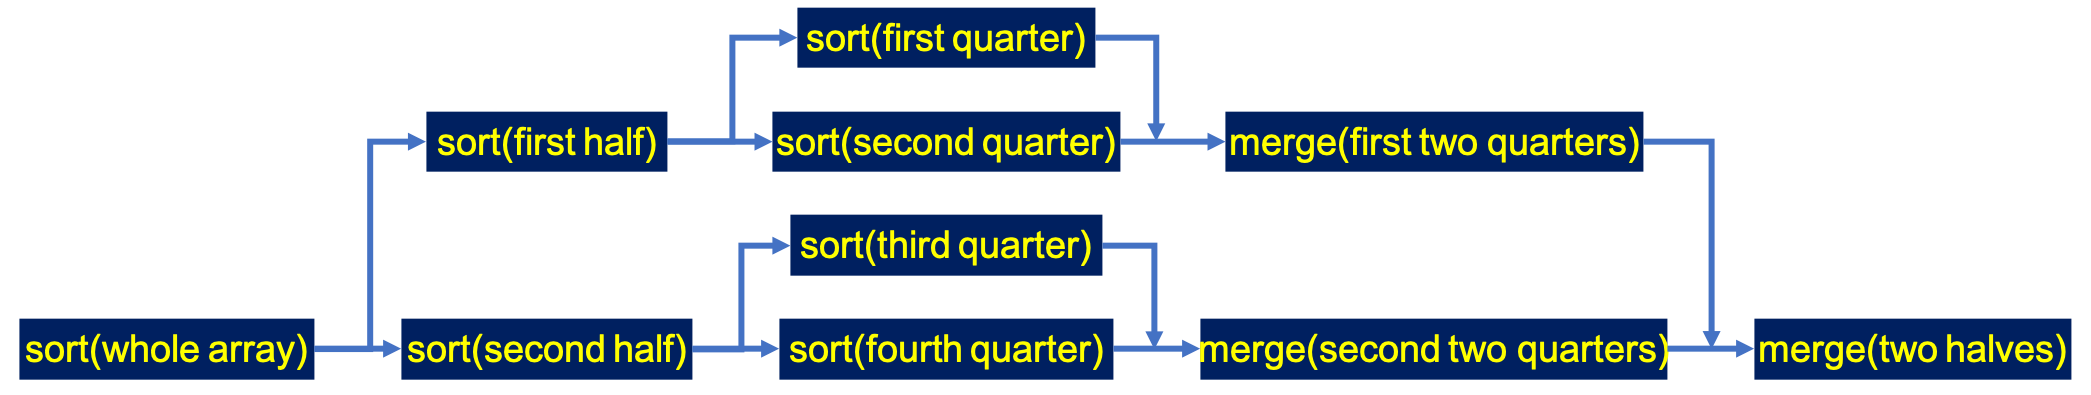
\includegraphics[scale=0.5]{mergesort-graph}

Compile \textit{mergesort.c} with \texttt{make mergesort}. The
\textit{mergesort} executable takes three arguments: a file containing integers
to be sorted (we have provided \textit{input.txt} which contains 30,000
integers), how many numbers should be read from the input file, and the number
of threads to use (with a little thought, you'll understand why the number of
concurrent flows of control often will be a power-of-two for Parallel Mergesort
-- but it doesn't need to be a power-of-two). The program will then sort the
list using the traditional Mergesort algorithm and then using Parallel
Mergesort, and it will then compare the performance of the two. Note that
\textit{mergesort.c} is written to measure time by the number of clock cycles
used and not by ``wall clock time.'' If we truly wanted to measure the
performance improvement, we would use ``wall clock time,'' but we are using
clock cycles used by the mergesort program so that we can ignore the
performance impact of other people using \runtimeenvironment at the same time
we are. For now, when you compile the program, you may get warnings for some
unused variables because the code to compare performance is commented-out while
we focus on getting the program to execute correctly.

Archie is unhappy that \function{parallel_mergesort} doesn't work quite right.
For example, if he tries to sort the first ten lines of \textit{input.txt},
only part of the list is sorted by \function{parallel_mergesort}:

\begin{verbatim}
labs> ./mergesort input.txt 10 2
 29722   9184   20537   13108   10423   20510   737   535   8040   25160
 535 < 737 < 8040 < 9184 < 10423 < 13108 < 20510 < 20537 < 25160 < 29722
 535 < 737 < 8040 < 20510 < 25160 < 29722 > 9184 < 20537 > 13108 > 10423
\end{verbatim}
The first line of the output is the list of numbers to be sorted; the second
line is the result of \function{sequential_mergesort}, and the third line is
the result of \function{parallel_mergesort}.

Your first task is to understand why only part of the list is sorted and to add
a line of code to make \function{parallel_mergesort} function correctly.

\section{Measuring Parallel Performance}

Open \textit{mergesort-analysis.xlsx}. The performance curve in the ``Chart1''
tab shows the ideal performance curve for Parallel Mergesort. In practice, the
performance gained would be less than ideal because part of the algorithm is
inherently sequential and also due to interprocess communication. When running
this implementation of \textit{mergesort.c} on \runtimeenvironment,
interprocess communication is negligible, and all else being equal the
sequential portion of the algorithm might reduce the performance gained but the
performance curve would retain its general shape.

Edit \textit{mergesort.c} and find the end of the \function{main} function. You
will see these lines:
\begin{lstlisting}
/*
    fprintf(stderr, "Parallel mergesort with %d threads executed %f times faster than sequential mergesort.\n", threadcount,
            (sequential_stop - sequential_start) / (parallel_stop - parallel_start));
*/
    return 0;
}
\end{lstlisting}
Un-comment the \lstinline{fprintf()} call and run re-compile the program. Now
when you run the program, it will output the measured performance
gain:\footnote{In chapter~10 we will see why the program might report a
performance gain with only one thread.}
\begin{verbatim}
labs> ./mergesort input.txt 10 1
 29722   9184   20537   13108   10423   20510   737   535   8040   25160
 535 < 737 < 8040 < 9184 < 10423 < 13108 < 20510 < 20537 < 25160 < 29722
 535 < 737 < 8040 < 9184 < 10423 < 13108 < 20510 < 20537 < 25160 < 29722
Parallel mergesort with 1 threads executed 2.300000 times faster than sequential mergesort.
\end{verbatim}

The shell script \textit{measure-mergesort.sh} will run \textit{mergesort}
several times so that we can use the average of several runs to measure the
performance gain, and it will discard all output except the performance report.
Run the shell script:
\begin{verbatim}
labs> ./measure-mergesort.sh
\end{verbatim}

Copy the shell script's output to your computer's clipboard. In
\textit{mergesort-analysis.xlsx}, place your cursor in cell A1 of the
``Sheet1'' tab and paste the shell script's output (it should overwrite cells
A1-A25). Go back to the ``Chart1'' tab and look at the performance curve. Does
the curve surprise you? Think of an explanation for why the performance curve
looks like it does.

In cell J2 of the ``Sheet1'' tab, type your explanation. (To receive credit,
your explanation does not have to be correct; your explanation only needs to be
plausible.) Be sure to save \textit{mergesort-analysis.xlsx}.

\section{Controlling Threads, part 2}

While Archie's idea to run parallel algorithms on the existing server didn't
pan out, you think he might be onto something with his next idea. Each source
of revenue (such as admissions gates) and each source of expense (such as
customer service) reports their individual gain/loss (in Zorkmids) at the end
of the day, after which their individual logs have to be consolidated into a
single ledger. It isn't until the next morning before unpleasant trends can be
detected, such as a sudden demand for refunds from zoo visitors who were
recently at the dire wolf feeding pen. (You involuntarily glance at the
magazine article you just finished.) If the revenues and expenses were recorded
into the shared ledger as they're generated, then it would be possible to
detect problems earlier.

In \textit{bookkeeper.c}, the \function{revenue_expense_generator} function
simulates the generation of revenues and expenses, prints them to the console,
and records them concurrently to the shared ledger. The \function{accounting}
function audits the ledger by reading the shared ledger. The ledger is an array
shared by all threads. By default, it has 2048 entries; however, you can
specify a smaller ledger with a command-line argument.

Compile the bookkeeper with \texttt{make bookkeeper}. When you run the
\textit{bookkeeper} executable, it will run the simulation until either the
ledger is full or you press Control-C.

After using the program for a few days, the Pleistocene Petting Zoo's
accountant calls an urgent meeting. While no safety issues were detected, the
accountant's daily audit of the ledger shows a discrepancy. For example:

\begin{verbatim}
labs> ./bookkeeper 50
Ledger is a 25-entry linear buffer
Created thread 139957550180096 for Admissions-1
Created thread 139957541787392 for Admissions-2
Created thread 139957533394688 for Admissions-3
1616975920855479130 (0) - visitor buys admission at gate 1, 10zm
1616975920855480807 (1) - visitor buys admission at gate 2, 10zm
1616975920855541055 (3) - refund issued at Customer Service, -11zm
Created thread 139957525001984 for Customer Service
1616975920855479962 (1) - visitor buys admission at gate 3, 10zm
Created thread 139957516609280 for Accountant
	Accounting reviews ledger (0) - visitor buys admission at gate 1, 10zm
	Accounting reviews ledger (1) - visitor buys admission at gate 3, 10zm
1616975920913184655 (4) - visitor buys admission at gate 2, 10zm
1616975920919503738 (5) - visitor buys admission at gate 1, 10zm
1616975920932387438 (6) - visitor buys admission at gate 3, 10zm
	Accounting reviews ledger (2) - (null), 0zm
1616975920970982633 (7) - visitor buys admission at gate 2, 10zm
1616975920983633203 (8) - visitor buys admission at gate 1, 10zm
1616975921009314194 (9) - visitor buys admission at gate 3, 10zm
	Accounting reviews ledger (3) - refund issued at Customer Service, -11zm
1616975921028728260 (10) - visitor buys admission at gate 2, 10zm
1616975921047694215 (11) - visitor buys admission at gate 1, 10zm
	Accounting reviews ledger (4) - visitor buys admission at gate 2, 10zm
1616975921086387242 (12) - visitor buys admission at gate 3, 10zm
1616975921086489603 (13) - visitor buys admission at gate 2, 10zm
1616975921111793869 (14) - visitor buys admission at gate 1, 10zm
	Accounting reviews ledger (5) - visitor buys admission at gate 1, 10zm
1616975921144081770 (15) - visitor buys admission at gate 2, 10zm
1616975921163343782 (16) - visitor buys admission at gate 3, 10zm
	Accounting reviews ledger (6) - visitor buys admission at gate 3, 10zm
1616975921175824363 (17) - visitor buys admission at gate 1, 10zm
1616975921201791056 (18) - visitor buys admission at gate 2, 10zm
	Accounting reviews ledger (7) - visitor buys admission at gate 2, 10zm
1616975921240001176 (19) - visitor buys admission at gate 1, 10zm
1616975921240240888 (20) - visitor buys admission at gate 3, 10zm
1616975921259427968 (21) - visitor buys admission at gate 2, 10zm
	Accounting reviews ledger (8) - visitor buys admission at gate 1, 10zm
1616975921304147073 (22) - visitor buys admission at gate 1, 10zm
Thread 139957550180096 terminated.
Thread 139957541787392 terminated.
Thread 139957533394688 terminated.
Thread 139957525001984 terminated.
Thread 139957516609280 terminated.
	Accounting reviews ledger (9) - visitor buys admission at gate 3, 10zm
	Accounting reviews ledger (10) - visitor buys admission at gate 2, 10zm
	Accounting reviews ledger (11) - visitor buys admission at gate 1, 10zm
	Accounting reviews ledger (12) - visitor buys admission at gate 3, 10zm
	Accounting reviews ledger (13) - visitor buys admission at gate 2, 10zm
	Accounting reviews ledger (14) - visitor buys admission at gate 1, 10zm
	Accounting reviews ledger (15) - visitor buys admission at gate 2, 10zm
	Accounting reviews ledger (16) - visitor buys admission at gate 3, 10zm
	Accounting reviews ledger (17) - visitor buys admission at gate 1, 10zm
	Accounting reviews ledger (18) - visitor buys admission at gate 2, 10zm
	Accounting reviews ledger (19) - visitor buys admission at gate 1, 10zm
	Accounting reviews ledger (20) - visitor buys admission at gate 3, 10zm
	Accounting reviews ledger (21) - visitor buys admission at gate 2, 10zm
	Accounting reviews ledger (22) - visitor buys admission at gate 1, 10zm
Revenue/Expense Report
        Admissions-1           80zm
        Admissions-2           80zm
        Admissions-3           60zm
    Customer Service          -11zm
                       ------------
Total gains/losses:           209zm
Accounting crosscheck:        199zm
\end{verbatim}

``There's a 10 Zorkmid discrepancy between what the zoo staff reports and
what's recorded in the ledger!'' the accountant frets. ``But it only happens
sometimes.''

``Don't worry,'' you reassure the accountant, ``nobody is embezzling. There's a
bug in the software, and I'll fix it.''

Your task is to identify the reason that the gains/losses value obtained by
summing the values calculated by the individual revenue/expense generators, and
the gains/losses obtained by summing the individual ledger entries, don't
always match. Once you have done that, add code to the program to correct the
problem.

Your solution must satisfy these properties:
\begin{itemize}
\item It must be functionally correct; that is, you must have solved the
    problem that the accountant discovered.
    \begin{itemize}
    \item The grader should be able to change parameters such as
        \lstinline{TIME_SCALE}, the number of threads running
        \function{revenue_expense_generator}, the number of threads running
        \function{accounting}, and the values in the \lstinline{pauses} array
        without affecting the correctness of your solution.
    \end{itemize}
\item A revenue/expense generator must be able to write to the ledger as soon
    as it has a revenue or expense to record, unless there is a good reason to
    force it to wait. Similarly, the accountant must be able to read from the
    ledger as soon as it is ready to do so, unless there is a good reason to
    force it to wait.
    \begin{itemize}
    \item No thread should be forced to wait simply because another
        thread is sleeping.
    \item As a special case of this requirement, you will receive no credit for
        this part of the assignment if your solution is to rewrite
        \textit{bookkeeper.c} to be a non-concurrent program.
    \end{itemize}
\end{itemize}

\section*{Turn-in and Grading}

When you have completed this assignment, upload \textit{mergesort.c},
\textit{mergesort-analysis.xlsx}, and {bookkeeper.c} to \filesubmission.

This assignment is worth 25 points. \\

\begin{description}
\rubricitem{5}{Parallel Mergesort functions correctly.}
\rubricitem{1}{Measured \textit{mergesort}'s performance, producing an actual performance curve.}
\rubricitem{4}{Arrived at a plausible explanation for \textit{mergesort}'s performance curve.}
\rubricitem{3}{Student demonstrates through their code that they know what \textit{bookkeeper}'s problem is, even if they don't correct it properly.}
\rubricitem{5}{A revenue/expense generator cannot unsafely write to the ledger.}
\rubricitem{4}{An accountant cannot unsafely read from the ledger.}
\rubricitem{3}{If a thread is ready to access the ledger and all other threads are sleeping, that thread is able to access the ledger.}
\end{description}

\end{document}
